\chapter{Gyakorlati megvalósítás}
\label{ch:gyakorlat}

A \textit{RelNorm} fejlesztéséhez \textit{Java} programnyelvet használtunk. Ezt a döntést kisebb elemzés előzte meg, amikor arra kerestük a választ, hogy milyen előnyökkel jár a \textit{Java} programnyelv használata ilyen probléma megoldásához. Kétségkívül objektum-orientált programnyelvet helyeztünk előtérbe, hiszen a funkcionális függőségek és attribútumok léte igazolja a különböző objektumok létét a rendszerünkben. Mindez mellett ezeket az objektumokat kollekciókba (halmazokba) kell rendeznünk, ezért egy objektum-orientált nyelv tűnt ígéretesnek a megvalósításhoz. A \textit{Java} programnyelv \lstinline{equals}, \lstinline{hashCode} és \lstinline{toString} beépített metódusainak használata is pozitívumot hozott a fejlesztéshez. A \textit{Java} programnyelv 8-as verziójától \textit{adatfolyamot} \index{adatfolyam (ang. \textit{stream})} is alkalmazni lehet, amely különféle szűréseket, átképzéseket, kalkulációkat és egyéb kollekciókon való műveleteket is engedélyez.
További szempont volt egy automatizált kódépítő eszköz használata, amellyel könnyedén felépíthetjük, tesztelhetjük és lefuttathatjuk a programot. A \textit{Maven} eszközre esett a választás, mivel széleskörben elterjedt, és a számunkra megfelelő funkciókkal van ellátva.

\section{Osztálydiagram}

A \textit{RelNorm} fejlesztése az osztálydiagrammal (\ref{fig:class} ábra) kezdődött. Az osztálydiagramon -- az átláthatóság érdekében -- mellőztük a konstruktőrok és egyéb \lstinline{get}/\lstinline{set} metódusok leírását, valamint a már említett \textit{Java} beépített metódusokét is. A \lstinline{Label} és a \lstinline{LabelSet} osztályok elnevezése megegyezik az irodalomban használt elnevezésekkel: attribute és attribute set. A \lstinline{Set} interface a \lstinline{java.util} csomagból került felhasználásra.

\begin{figure}
    \centering
    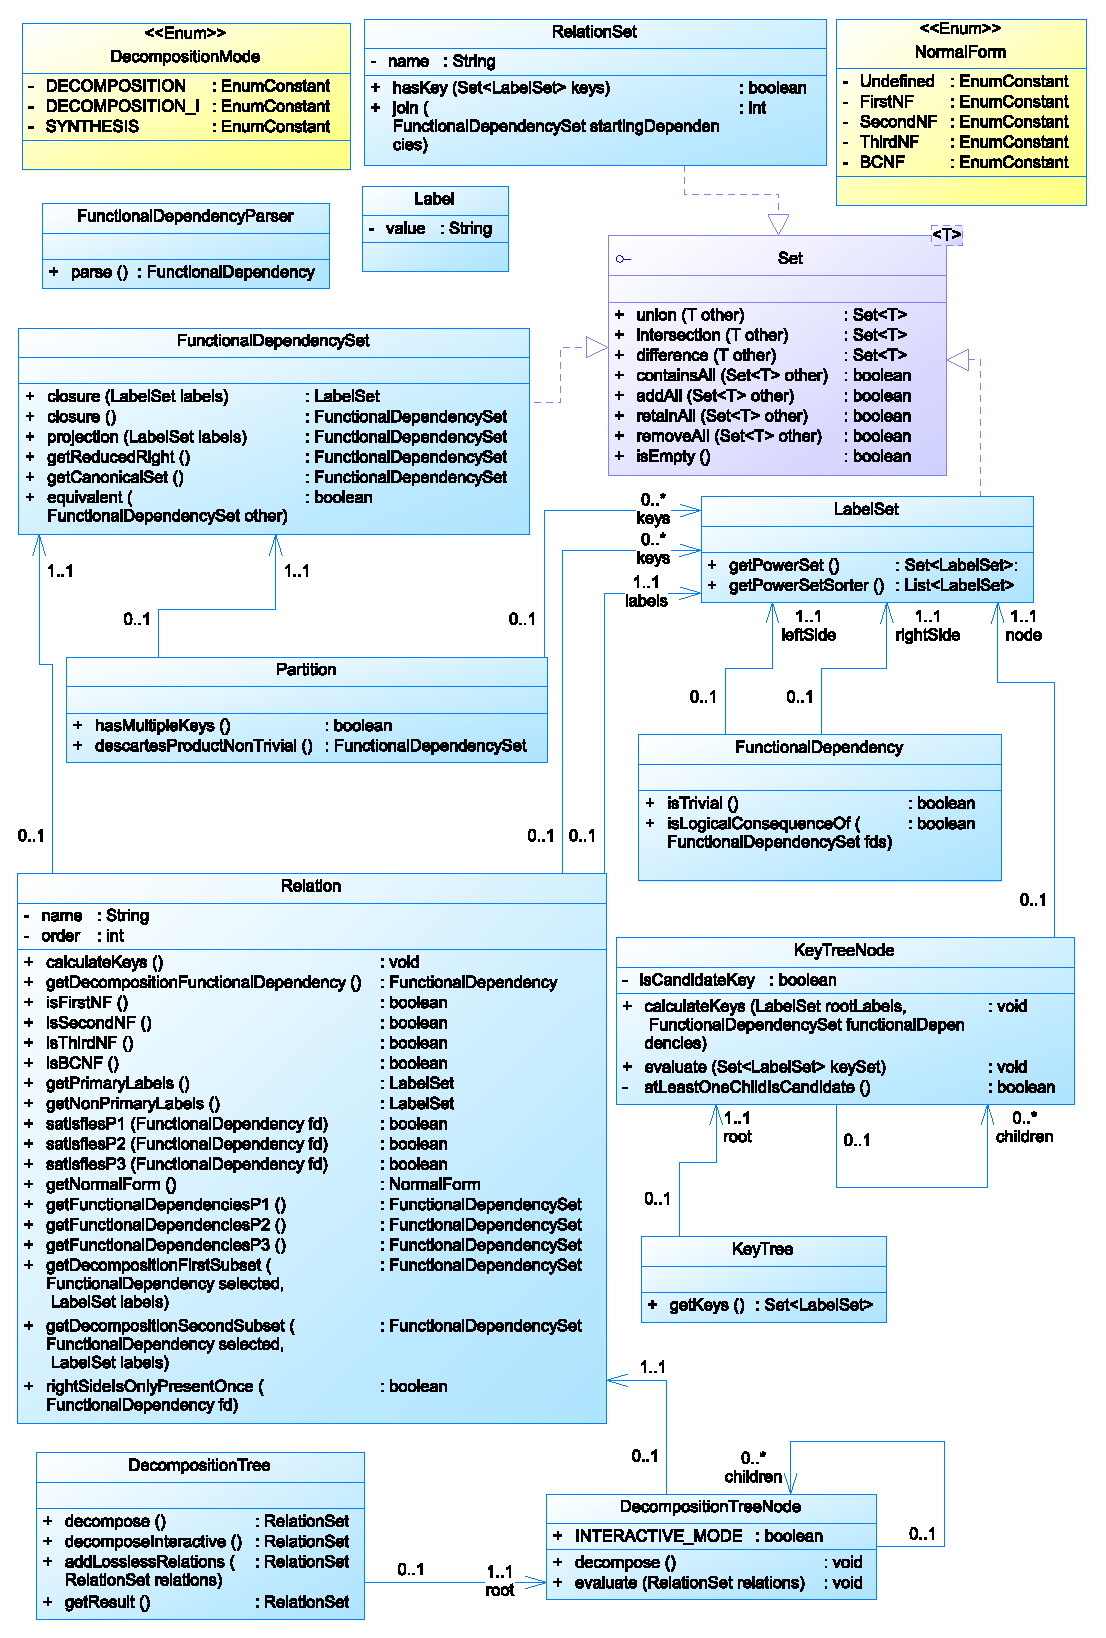
\includegraphics[width=1\textwidth]{ClassDiagram_1}
    \caption{\textit{RelNorm} osztálydiagram}
    \label{fig:class}
\end{figure}
 
\section{Alapvető algoritmusok/kódrészletek}

Ebben a részben az előző fejezetben leírt alapvető relációs fogalmak és műveletek algoritmusainak a megvalósítása kerül bemutatásra.

Az attribútumhalmaz lezártjának a definícióját (\ref{eq:closure} képlet) a függőséghalmaz \lstinline{closure} metódusával tudjuk kiszámolni:

\linespread{1}
\begin{lstlisting}[language=Java]
public LabelSet closure(LabelSet labels) {
	LabelSet result = new LabelSet(labels);
	LabelSet lastResult;
	do {
		lastResult = new LabelSet(result);

		this.items.forEach(fd -> {
			if(result.containsAll(fd.getLeftSide())) {
				result.addAll(fd.getRightSide());
			}
		});
	} while(!lastResult.equals(result));
	return result;
}
\end{lstlisting}

A függőséghalmaz projekcióját (\ref{eq:projection} képlet) a függőséghalmaz \lstinline{projection} metódusával tudjuk kiszámolni:

\linespread{1}
\begin{lstlisting}[language=Java]
public FunctionalDependencySet projection(LabelSet labels) {
	FunctionalDependencySet projection = new FunctionalDependencySet();
	for(LabelSet subset: labels.getPowerSet()) {
		LabelSet closure = this.closure(subset);
		closure.retainAll(labels);
		closure.removeAll(subset);
		if(!closure.isEmpty()) {
			FunctionalDependency fd = 
			    new FunctionalDependency(subset, closure);
			projection.add(fd);
		}
	}
	return projection;
}
\end{lstlisting}

A fenti kódrészletben szerepel egy \lstinline{getPowerSet} nevezetű metódus, amely egy adott attribútumhalmaz összes részhalmazának a halmazát számolja ki \parencite{baeldung2020}.

Az igaz következmény, azaz egy függőséghalmazhoz viszonyított függőség logikai következényének a definícóját (\ref{eq:setclosure} képlet) az attribútumhalmaz \lstinline{isLogicalConsequenceOf} metódusával lehet kiszámolni.

\linespread{1}
\begin{lstlisting}[float,floatplacement=H,language=Java]
public boolean isLogicalConsequenceOf(FunctionalDependencySet dependencies) {
	LabelSet closure = dependencies.closure(leftSide);
	return closure.containsAll(rightSide);
}
\end{lstlisting}

Két függőséghalmaz egybevágóságát (\ref{eq:equiv} képlet) a függőséghalmaz equivalent metódusa számolja ki.

\linespread{1}
\begin{lstlisting}[float,floatplacement=H,language=Java]
public boolean equivalent(FunctionalDependencySet other) {
	return 
		this.stream().allMatch(fd -> fd.isLogicalConsequenceOf(other)) &&
		other.stream().allMatch(fd -> fd.isLogicalConsequenceOf(this));
}
\end{lstlisting}

A relációs sémák kulcshalmazához az előző fejezetben leírt algoritmust (\ref{eq:reductionop} képlet) használjuk. A megvalósításhoz elengedhetetlen egy ún. \textit{kulcsfa} \index{kulcsfa (ang. \textit{key tree})} használata. Ez a kulcsfa olyan csomópontokból áll össze, melyek tartalmaznak egy atribútumhalmazt, információt a kulcsjelölti státuszukról valamint egy kollekciót a gyermekeiről. A gyermek csomópont pontosan egy attribútummal kevesebbet tartalmaz a szülőtől. Ha egy megadott attribútumhalmaz $U=\{A,B,C,D\}$ és függőséghalmaz $F=\{AC \to B,BC \to D,A \to B,B \to A\}$ kulcsait szeretnénk megkapni ($K=\{AC,BC\}$), akkor a(z) \ref{fig:keytree} ábra mutatja be ennek a példának a kulcsfáját.

\begin{figure}
    \centering
    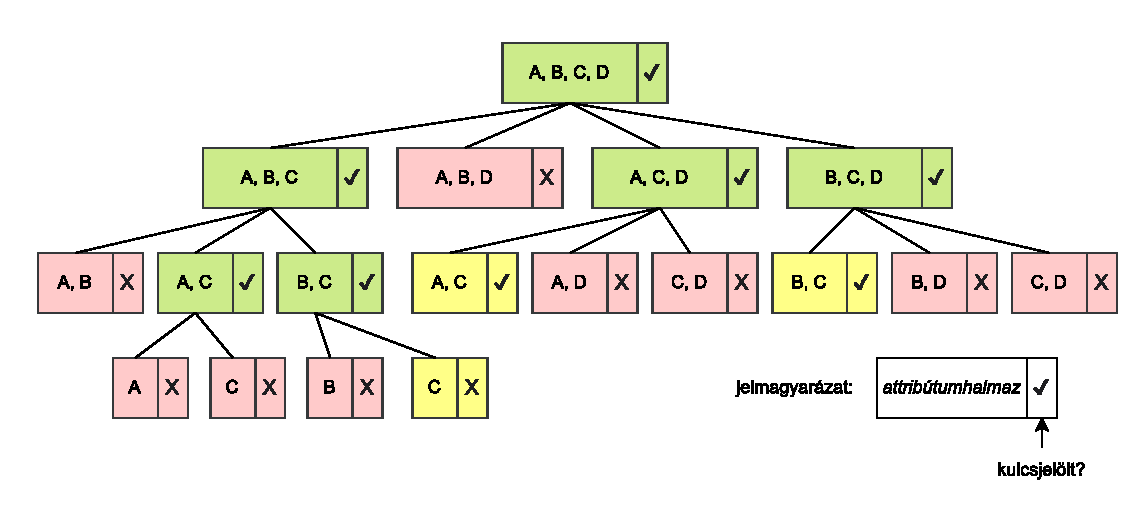
\includegraphics[width=1\textwidth]{keytree}
    \caption{Kulcsfa}
    \label{fig:keytree}
\end{figure}

A zölddel jelölt csomópontokat további rekurzív számításnak vetjük alá mindaddig, amíg egy csomópont kulcsjelölti státusza meg nem szűnik (piros) vagy már az adott csomópont attribútumhalmazát bejártuk (sárga). A kulcsfa kiértékelésénél azokat a zöld csomópontokat tekintjük kulcsnak, amelyek kulcsjelöltek, de egyik gyermekük sem kulcsjelölt.

\section{Normálformák megvalósítása}

Az első normálforma, azaz az \textit{1NF} előzetes megegyezés szerint mindig teljesítve lesz, mivel a normalizációs algoritmusok nem tudják megállapítani egyes attribútumok struktúráját.

\linespread{1}
\begin{lstlisting}[language=Java]
public boolean isFirstNF() {
	return true;
}
\end{lstlisting}

Az első normálformán túl szükségünk van további kisegítő metódusokra. Ilyen metódusok a primáris és szekundáris attribútumhalmazt kiszámoló metódusok. A primáris attribútumok a \lstinline{getPrimaryLabels} metódussal kaphatóak meg.

\linespread{1}
\begin{lstlisting}[language=Java]
private LabelSet getPrimaryLabels() {
	LabelSet primaryLabels = new LabelSet();
	keys.forEach(primaryLabels::addAll);
	return primaryLabels;
}
\end{lstlisting}

A szekundáris attribútumok a \lstinline{getNonPrimaryLabels} metódussal kaphatóak meg.

\linespread{1}
\begin{lstlisting}[language=Java]
private LabelSet getNonPrimaryLabels() {
	LabelSet allLabels = new LabelSet(labels);
	allLabels.removeAll(getPrimaryLabels());
	return allLabels;
}
\end{lstlisting}

A reláció \lstinline{isSecondNF} metódusával kapjuk meg azt az információt, hogy egy adott reláció teljesíti-e a \textit{2NF} normálformát annak definíciója szerint (\ref{eq:2nf} képlet).

\linespread{1}
\begin{lstlisting}[language=Java]
public boolean isSecondNF() {
    LabelSet nonPrimaryLabels = getNonPrimaryLabels();
    if(nonPrimaryLabels.isEmpty()) {
        return true;
    }

    return getKeys().stream().allMatch(key -> {
        Set<LabelSet> subsets = key.getSubsets();
        return subsets.stream().allMatch(subset -> 
            nonPrimaryLabels.stream().noneMatch(nonPrimaryLabel ->
                functionalDependencies.closure(subset)
                    .contains(nonPrimaryLabel)));
    });
}
\end{lstlisting}

A \textit{3NF} normálformának az alternatív definíciója alapján (\ref{eq:3nfalt} képlet) készült el a relációs séma \lstinline{isThirdNF} metódusa.

\linespread{1}
\begin{lstlisting}[language=Java]
public boolean isThirdNF() {
	LabelSet nonPrimaryLabels = getNonPrimaryLabels();
	if(nonPrimaryLabels.isEmpty()) {
		return true;
	}

	return functionalDependencies.stream().allMatch(fd -> {
		if(nonPrimaryLabels.containsAll(fd.getRightSide())) {
			return getKeys().stream().anyMatch(key -> 
				fd.getLeftSide().containsAll(key));
		} else {
			return true;
		}
	});
}
\end{lstlisting}

A \textit{BCNF} normálforma definíciója (\ref{eq:bcnf} képlet) alapján létrejött \lstinline{isBCNF} metódussal számítható ki, hogy egy relációs séma teljesíti-e a \textit{BCNF} normálformát.

\linespread{1}
\begin{lstlisting}[language=Java]
public boolean isBCNF() {
	return functionalDependencies.stream()
		.filter(fd ->!fd.isTrivial())
		.allMatch(fd -> getKeys().stream().
			anyMatch(key -> fd.getLeftSide().containsAll(key)));
}
\end{lstlisting}

Tekintettel a \ref{eq:nf} képletekre, egy bizonyos relációs séma normálformájának a megállapítását a \lstinline{getNormalForm} metódussal valósítottuk meg.

\linespread{1}
\begin{lstlisting}[language=Java]
public NormalForm getNormalForm() {
	return isBCNF() ? NormalForm.BCNF :
     			isThirdNF() ? NormalForm.ThirdNF :
				isSecondNF() ? NormalForm.SecondNF :
					isFirstNF() ? NormalForm.FirstNF : 
						NormalForm.Undefined;
}
\end{lstlisting}

\section{Szintézis algoritmusának a megvalósítása}

A szintézis algoritmusának számítógépes megvalósítását a(z) \ref{fig:synseq} ábra tükrözi. Felhasználói beavatkozás, ami befolyásolná az algoritmus kimenetelét, nem történik a lefuttatás alatt.

\begin{figure}
    \centering
    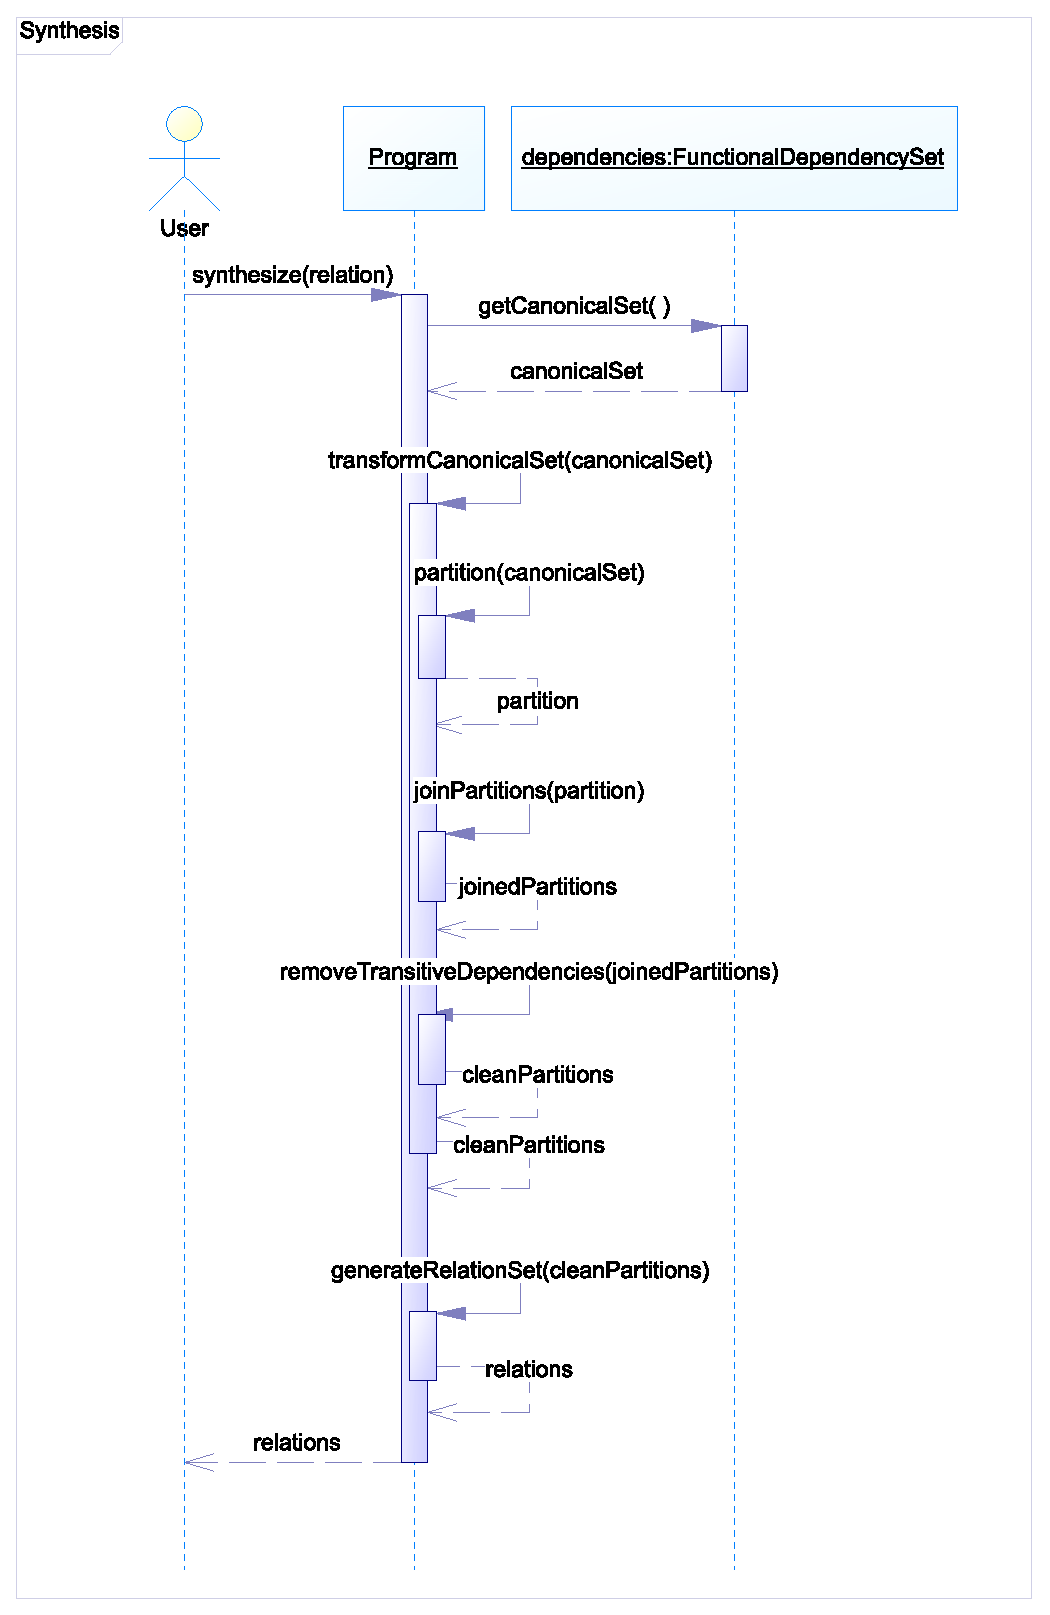
\includegraphics[width=0.95\textwidth]{Synthesis}
    \caption{A szintézis szekvenciadiagramja}
    \label{fig:synseq}
\end{figure}

A szintézis algoritmusa alapján a legfontosabb lépés a minimális függéshalmaz kiszámolása. Ezt három lépésből tudjuk megtenni: A minimális függéshalmazban a függőségek jobboldali attribútumhalmazában csak egyetlen attribútum található (\ref{eq:syn1-2} képlet), a függőségek teljes függőségek (\ref{eq:syn1-3} képlet), valamint nincs olyan függőség, amelyik elhagyható (\ref{eq:syn1-4} képlet).

\begin{enumerate}

    \item A jobboldali függőségek egy atribútummá való redukálása:
    
\linespread{1}
\begin{lstlisting}[language=Java]
FunctionalDependencySet reduced = new FunctionalDependencySet();
items.forEach(
	fd -> fd.getRightSide().forEach(
		label -> reduced.add(
			new FunctionalDependency(fd.getLeftSide(), label))
	)
);
\end{lstlisting}

    \item A részleges függőségek teljes függésé való átalakítása
    
\linespread{1}
\begin{lstlisting}[language=Java]
FunctionalDependencySet reducedS = new FunctionalDependencySet(canonicalSet);
reduced.forEach(
	fd -> fd.getLeftSide().getPowerSetSorted().stream()
	.filter(subset -> !subset.isEmpty() && !subset.equals(fd.getLeftSide()))
	.map(subset -> new FunctionalDependency(subset, fd.getRightSide()))
	.filter(partial -> partial.isLogicalConsequenceOf(reducedS))
	.limit(1)
	.forEach(partial -> {
		reducedS.add(partial);
		reducedS.remove(fd);
	})
);
\end{lstlisting}

    \item Elhagyható függőségek törlése
    
\linespread{1}
\begin{lstlisting}[language=Java]
FunctionalDependencySet setToRemove = new FunctionalDependencySet();
reducedS.stream()
	.filter(fd ->
		fd.isLogicalConsequenceOf(
			reducedS.difference(fd).difference(setToRemove)))
	.forEach(setToRemove::add);
reducedCanonicalSet.removeAll(setToRemove);
\end{lstlisting}
\end{enumerate}

A partíciók kialakításához először egy \lstinline{HashMap} kollekcióba rendeztük a függőségeket, a baloldali attribútumhalmazaitól függően. Ezután ezeknek a baloldali attribútumhalmazoknak kiszámoltuk a zártját, és amennyiben azok megegyeztek, összevontuk ezeket a partíciókat. Ezek az algoritmusok viszonylag egyszerűek, ezért nem kerülnek bemutatásra ebben a dolgozatban.

Ezután következik az összevonás által keletkezett potenciálisan tranzitív függőségek eltávolítása a partíciókból. Ennek kiszámolása érdekében a következőképpen létrehozzuk a $J$ függőséghalmazt (\ref{eq:syn2-6} képlet).

\linespread{1}
\begin{lstlisting}[language=Java]
FunctionalDependencySet jay = new FunctionalDependencySet();
for(Partition partition: partitions) {
	FunctionalDependencySet desc = partition.descartesProductNonTrivial();
	FunctionalDependencySet descReduced = descartes.getReducedRight();
	jay.addAll(descReduced);
	partition.removeAll(descReduced);
}
\end{lstlisting}

A \lstinline{descartesProductNonTrivial} metódus kiszámolja az összevont partícióknak az ún. permutációs (nem triviális) függőséghalmazát (\ref{eq:syn2-7} képlet). Azaz, ha $A$, $B$ és $C$ kulccsal rendelkező partíciókat vontunk össze, akkor ez a metódus eredményként $A \to B$, $B \to A$, $A \to C$, $C \to A$, $B \to C$ és $C \to B$ függőségeket eredményezi. Majd ezeken a függőségeken jobb oldali egyszerűsítést végzünk annak érdekében, hogy a jobboldali attribútumhalmaz csak egy attribútumot tartalmazzon.

A tranzitív függőségek eltávolításához befejező lépésként megalkotjuk az $M$ függőséghalmazt (\ref{eq:syn2-8} képlet).

\linespread{1}
\begin{lstlisting}[language=Java]
FunctionalDependencySet em = new FunctionalDependencySet();
em.addAll(jay);
partitions.forEach(p -> em.addAll(p.getValues()));

partitions.forEach(partition -> {
	FunctionalDependencySet functionalDependenciesCopy =
		new FunctionalDependencySet(partition.getValues());
		functionalDependenciesCopy.forEach(fd -> {
    public ChannelService(ChannelRepository repository, OrganizationService organizationService, FilesystemUtil fsUtil) {
        this.repository = repository;
        this.organizationService = organizationService;
        this.fsUtil = fsUtil;
    }
			if(fd.isLogicalConsequenceOf(em.difference(fd))) {
				partition.remove(fd);  // fd is transitive dependency
			}
		});
});

partitions.forEach(partition -> partition.addAll(jay));
\end{lstlisting}

A relációs séma halmaza a szintézis algoritmusa alapján megfelel a létrejött partícióknak, amit így alkotunk meg:

\linespread{1}
\begin{lstlisting}[language=Java]
RelationSet relations = new RelationSet("S");
int n = 1;
for(Partition partition : partitions) {
	LabelSet labels = partition.getLabels();
	Relation relation = 
		new Relation("S", n++, labels, partition.getValues());
	relations.add(relation);
}
\end{lstlisting}

A veszteségmentes sémafelbontást érdekében a kezdetleges relációs séma egyik kulcsát tartalmazó relációs sémát hozunk létre, amennyiben olyan relációs séma nem képezi az eddig létrejötteket:

\linespread{1}
\begin{lstlisting}[language=Java]
if(!relations.hasKey(initialRelation.getKeys())) {
	Relation lossless = 
		new Relation("S", n, 
			initialRelation.getKeys().stream().findAny().get(),
			new FunctionalDependencySet());
	relations.add(lossless);
}
\end{lstlisting}

\section{Dekompozíció algoritmusának a megvalósítása}

A dekompozíció első lépése a megfelelő függőség kiválasztása. Ezt a függőséget háromféle kritérium alapján tudjuk kiválasztani. A következő metódusok azt vizsgálják, hogy egy adott függőség megfelel-e a P1 (\ref{eq:p1}), P2 (\ref{eq:p2}) illetve a P3 (\ref{eq:p3}) kritériumnak. 

\linespread{1}
\begin{lstlisting}[language=Java]
public boolean satisfiesP1(FunctionalDependency fd) {
	return !fd.isTrivial() &&
		keys.stream().noneMatch(k -> fd.getLeftSide().containsAll(k)) && 
		functionalDependencies.equivalent(
			functionalDependencies.projection(fd.getLeftSide()
				.union(labels.difference(fd.getRightSide())))
		.union(functionalDependencies.projection(fd.getLeftSide()
				.union(fd.getRightSide()))));
}
\end{lstlisting}

\linespread{1}
\begin{lstlisting}[language=Java]
public boolean satisfiesP2(FunctionalDependency fd) {
	return !fd.isTrivial() &&
		!fd.getLeftSide().union(fd.getRightSide()).containsAll(labels) &&
		functionalDependencies.equivalent(
			functionalDependencies.projection(fd.getLeftSide()
				.union(labels.difference(fd.getRightSide())))
			.union(functionalDependencies.projection(fd.getLeftSide()
				.union(fd.getRightSide()))));
}
\end{lstlisting}

\linespread{1}
\begin{lstlisting}[language=Java]
public boolean satisfiesP3(FunctionalDependency fd) {
	return !fd.isTrivial() && keys.stream().noneMatch(k ->
		fd.getLeftSide().containsAll(k));
}
\end{lstlisting}

A szintézis algoritmussal ellentétben, a dekompozíció algoritmusánál a felhasználó is beleszólhat az algoritmus lefolyásába. Ezt oly módon teszi, hogy a felkínált függőségekből (melyek lehetőleg minél nagyobb kritériumi szintet teljesítenek) választ egyet. A(z) \ref{fig:dectree} ábra bemutatja, hogy minderre a \lstinline{decompose} metódus elején kerül sor – a \lstinline{user selects functional dependency} üzenettel. Az algoritmus interaktív mivolta úgy valósul meg, hogy a program a standard kimenetre nyomtatja a választható függőségeket, a felhasználó pedig a billentyűzet segítségével kiválasztja a neki megfelelő függőséget. Az algoritmus automatikus változata ezt a választás lehetőségét átugorja, és találomra választ egy függőséget a felkínáltak közül.

Mivel a dekompozíció lépéseiben az algoritmus az aktuális relációs sémát két relációs sémára válassza szét (\ref{eq:r1r2} képlet), innen ered az ötlet, hogy a dekompozíció megvalósításához elég létrehozni egy ún. dekompozíciós fát. Ennek a fának a csomópontjai relációs sémák lesznek, a levelei pedig a dekompozíció eredményeként létrejött relációs sémahalmazt alkotják.

\begin{figure}
    \centering
    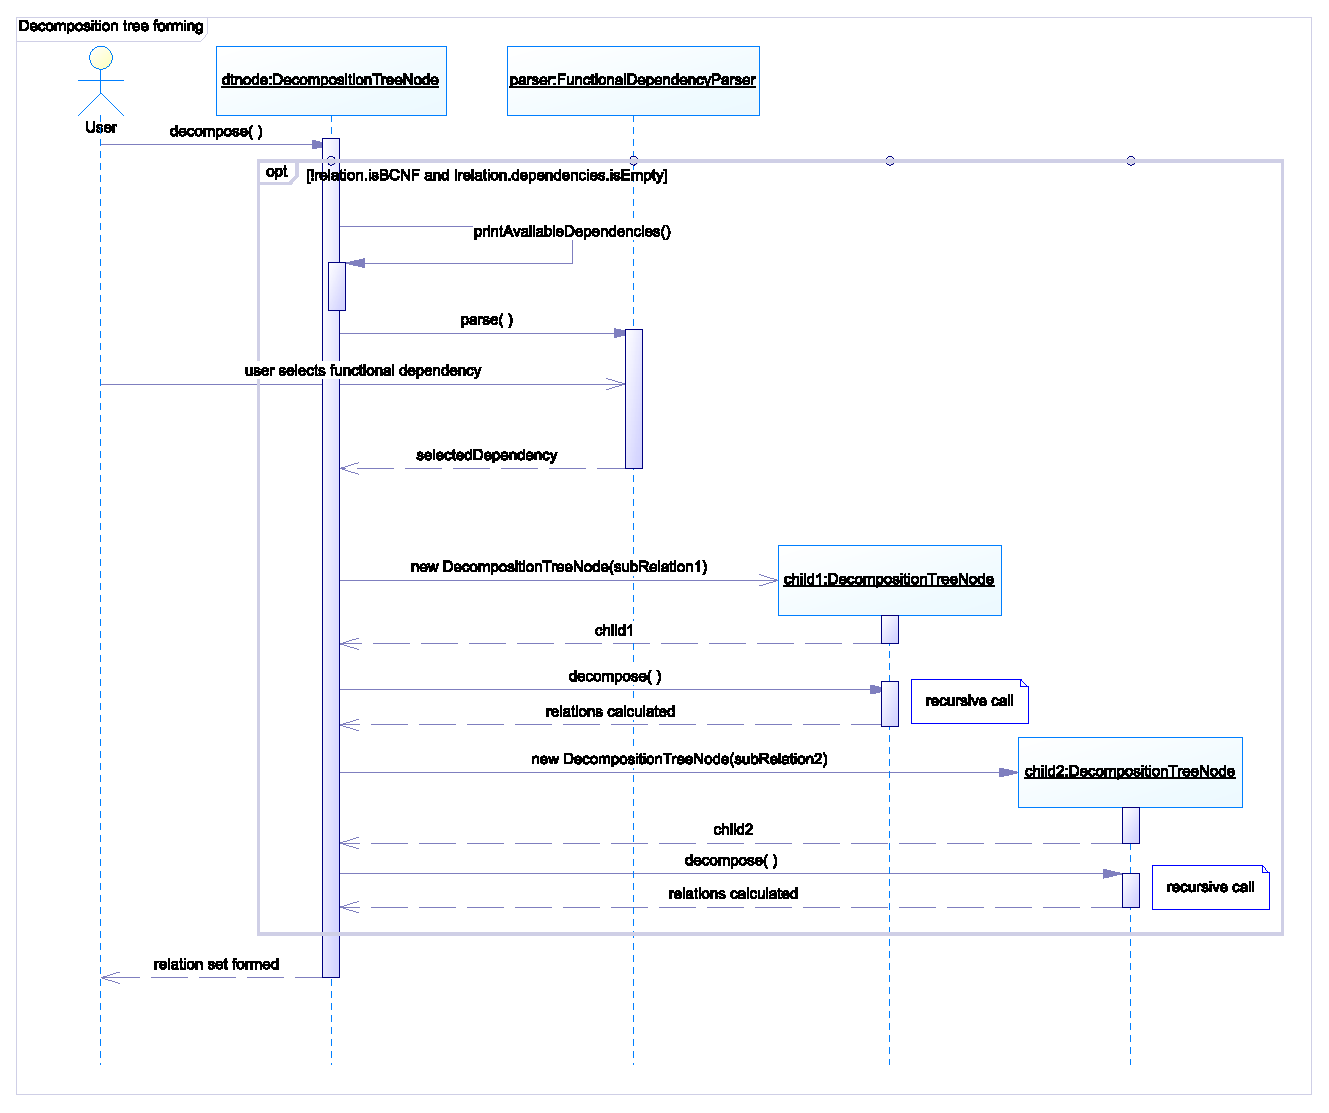
\includegraphics[width=1\textwidth]{Decomposition_tree_forming}
    \caption{A dekompozíciós fa formálásának a szekvenciadiagramja}
    \label{fig:dectree}
\end{figure}

A dekompozíciós fa létrejöttéhez a \lstinline{decompose} metódus rekurzív előhívása szükséges a relációs séma dekomponált gyermekcsomópontjain. Ez a folyamat addig folytatódik, amíg nem kapunk olyan relációs sémákat, amelyek teljesítik a \textit{BCNF} normálformát.

Miután létrehoztuk az ún. dekompozíciós fát, ki kell értékelni azt. Ezt szintén rekurzív módszerekkel oldottuk meg (\ref{fig:decomposition} ábra). A fa leveleinek a begyűjtése után ki kell vizsgálni, hogy az azonos kulcsokkal rendelkező relációs sémákat összevonjuk, majd leellenőrizzük a veszteségmentes sémafelbontás feltételeit. Ezt hasonlóképp végezzük el, mint a szintézis algoritmusa során. 

\begin{figure}
    \centering
    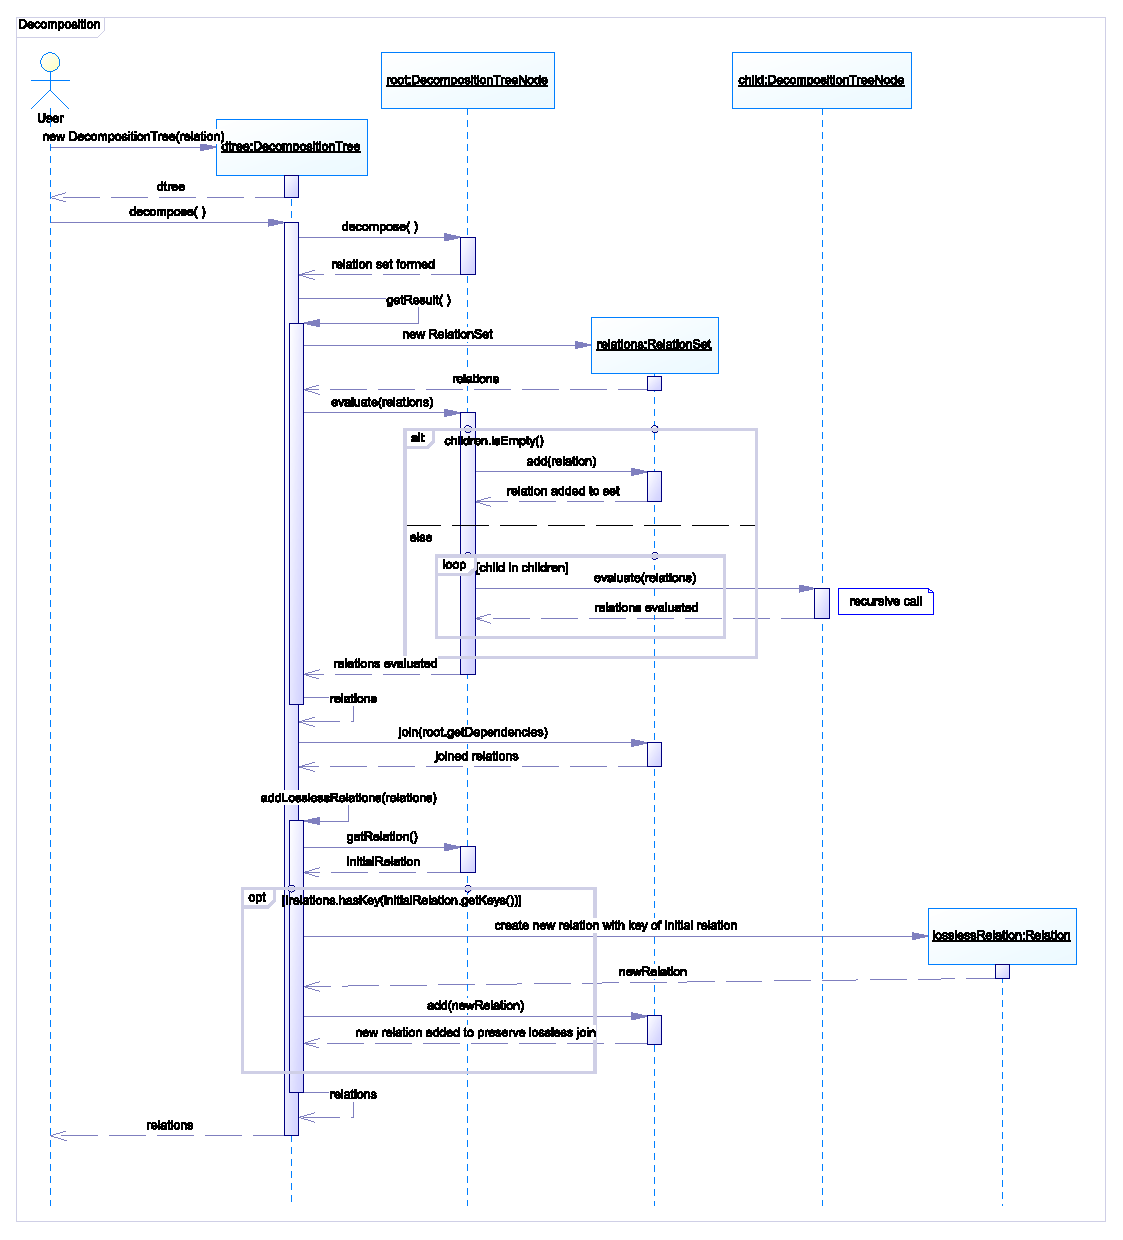
\includegraphics[width=1\textwidth]{Decomposition}
    \caption{A dekompozíciós fa kiértékelésének a szekvenciadiagramja}
    \label{fig:decomposition}
\end{figure}

\section{Egyéb magvalósítási részletek}

A dolgozatban felvázolt célkitűzések között szerepel az a követelmény, hogy a feladatsorok könnyen megadhatóak és cserélhetőek legyenek. Ennek a követelménynek tettünk eleget, hogy szöveges úton engedélyeztük a program bemeneti feladatsorát. A felhasználó egy \textit{JSON} típusú fájlként tudja megadni a feladatsorát, majd lefuttatáskor a megfelelő fájlt tudja bemenetként megadni.

Példaként szolgálva, ha egy $N$ nevezetű relációnak az attribútumhalmaza $\{A,B,C,D,E\}$, függőséghalmaza pedig $\{AB \to CE, C \to D\}$, akkor a bemeneti feladatsor fájlja a következőképp néz ki:

\linespread{1}
\begin{lstlisting}
{
  "name": "N",
  "labels": ["A", "B", "C", "D", "E"],
  "functionalDependencies": [
    {"left": ["A", "B"], "right": ["C", "E"]},
    {"left": ["C"], "right": ["D"]}
  ]
}
\end{lstlisting}

A forráskód felépítéséhez és becsomagolásához a \textit{Maven} eszköz \lstinline{package} parancsa szükséges:

\linespread{1}
\begin{lstlisting}[language=sh]
mvn package
\end{lstlisting}

A sikeres csomagolás után a build mappában fog szerepelni a \textit{JAR} csomag, melyet a következőképp tudunk lefuttatni:

\linespread{1}
\begin{lstlisting}[language=sh]
java -jar rel-norm-1.0-SNAPSHOT.jar <task> <method>
\end{lstlisting}

A \lstinline{<task>} megjelölés helyett a feladatsor fájljának az útvonalát kell megadni, a \lstinline{<method>} megjelölés helyett meg egyikét a következőnek:

\begin{itemize}
    \item \lstinline{DECOMPOSITION} -- a dekompozíció algoritmus lefuttatásához,
	\item \lstinline{DECOMPOSITION_I} -– a dekompozíció interaktív algoritmusának lefuttatásához és
	\item \lstinline{SYNTHESIS} -- a szintézis algoritmusának a lefuttatásához.
\end{itemize}
	
\section{Szoftvertesztek megvalósítása}

A \textit{Java} programnyelvnek rendeltetésszerű tesztelési munkakeretét használtuk a dolgozatban. A munkakeret neve \textit{JUnit}, ami unit-tesztek írását és lefuttatását teszi lehetővé. A dolgozat \ref{ch:elmelet}. fejezetében felsorolt relációs műveletek és algoritmusok mindegyike szerepel a teszt esetekben. A tesztek érvényességét feladatgyűjteményből \parencite{kordic2018} származtatott feladatok és megoldásaik szavatolják. A tesztek elindításához a következő parancsot kell végrehajtani:

\linespread{1}
\begin{lstlisting}[language=sh]
mvn test
\end{lstlisting}

A kód lefedettség kiszámolása érdekében külső szoftverelemző eszközt használunk. A \textit{SonarCloud} online kódbázis elemző szoftver, amivel git alapú kódbázisokat tudunk megfigyelni. A \textit{SonarCloud} képes jelenteni programhibákat, biztonsági réseket, nem tiszta kód jellemzőit, kód többszöröződést stb. Mindezek mellett még kód lefedettségi szintet is mér, habár ezt külső tesztjelentésből állítja össze. Ahhoz, hogy a \textit{SonarCloud} külső tesztjelentéseket tudjon olvasni, integrálni kell a \textit{JaCoCo} bővítményt a \textit{Maven} projektbe. Ez a bővítmény jelentéseket készít a lefuttatott tesztekről.
